\documentclass[preprint]{aastex}  % USE THIS TO MAKE BIB, THEN FORMAT USING EMULATEAPJ
%\documentclass[twocolumn,numberedappendix]{emulateapj}
\shorttitle{Transit Dish for 21cm Intensity Mapping}
\shortauthors{XXX Authors}

\usepackage{amsmath}
\usepackage{graphicx}
\usepackage[figuresright]{rotating}
%\usepackage{rotating}
\usepackage{natbib}
%\usepackage{pdflscape}
%\usepackage{lscape}
\citestyle{aa}

\newcommand{\BigO}[1]{\mathcal{O}(#1)}
\def\k{\mathbf{k}}
\def\r{\mathbf{r}}
\def\V{\mathbb{V}}
\def\At{\tilde{A}}
\def\Vt{\tilde{V}}
\def\Tt{\tilde{T}}
\def\tb{\langle T_b\rangle}

\begin{document}
\title{A Transit Dish Design for High-Redshift 21cm Intensity Mapping Experiments}

\author{
%Aaron R. Parsons\altaffilmark{1,2},
%Adrian Liu\altaffilmark{1},
%James E. Aguirre\altaffilmark{3},
%Zaki S. Ali\altaffilmark{1},
%Richard F. Bradley\altaffilmark{4,5,6},
%Chris L.  Carilli\altaffilmark{7},
%David R. DeBoer\altaffilmark{2},
%Daniel C. Jacobs\altaffilmark{8},
%David F. Moore\altaffilmark{3},
%Jonathan C. Pober\altaffilmark{1},
}

%\altaffiltext{1}{Astronomy Dept., U. California, Berkeley, CA}
%\altaffiltext{2}{Radio Astronomy Lab., U. California, Berkeley, CA}
%\altaffiltext{3}{Dept. of Physics and Astronomy, U. Pennsylvania, Philadelphia, PA}
%\altaffiltext{4}{Dept. of Electrical and Computer Engineering, U. Virginia, Charlottesville, VA}
%\altaffiltext{5}{National Radio Astronomy Obs., Charlottesville, VA}
%\altaffiltext{6}{Dept. of Astronomy, U. Virginia, Charlottesville, VA}
%\altaffiltext{7}{National Radio Astronomy Obs., Socorro, NM}
%\altaffiltext{8}{School of Earth and Space Exploration, Arizona State U., Tempe, AZ}
%\altaffiltext{9}{Square Kilometer Array, South Africa Project, Cape Town, South Africa}
%\altaffiltext{10}{Cavendish Lab., Cambridge, UK}

\begin{abstract}
\end{abstract}

\section{Introduction}

\begin{itemize}
\item importance of frequency smoothness
\item collecting area
\end{itemize}

\section{Background}
\label{sec:background}

\begin{itemize}
\item $\tau$-modes, wedge, EoR window
\item geometric interpretation of $\tau$-modes
\end{itemize}

\section{Geometric Constraints}
\label{sec:geometry}

\begin{itemize}
\item first principles of EoR window, how that maps to a specification for design
\item cost analysis
\item critically constrained design
\item symmetric on-axis parabaloid, for reasons of symmetry in polarization response
\end{itemize}

\section{Design and Construction}
\label{sec:design}

\subsection{bent pipes as approximation to parabola}

\begin{figure}[H]
	\begin{center}
	\includegraphics[width =\textwidth]{}
	\caption{THIS FIGURE SHOWS THE ANALYSIS ON PARABOLA
\label{Fig:} }
	\end{center}
\end{figure}


\subsection{faceting (rms deviation from parabaloid)}
\begin{figure}[H]
	\begin{center}
	\includegraphics[width =\textwidth]{}
	\caption{THIS FIGURE SHOWS THE PHOTGRAMMRY ANALYSIS 
\label{Fig:} }
	\end{center}
\end{figure}


\begin{itemize}
\item bent pipes as approximation to parabola 
\item faceting (rms deviation from parabaloid)  
\item shielding (screens)
\item splash cone
\item hub --> see technical doc
\item feed suspension (feed with mast, back screen by kevlar wire)
\item materials, PVC selection -> construction_journal.tex
\item design lifetime (wood, PVC)
\end{itemize}

\section{Simulated Performance}
\label{sec:sim}

\begin{itemize}
\item beam pattern
\item delay performance (E-M modeling)
\end{itemize}

\section{Fabrication and Deployment}
\label{sec:deploy}

\begin{itemize}
\item lessons/principles
\item process to precision to specifications on precision
\end{itemize}





\section{Reflectometry Test Setup}
\label{sec:reflect}
During the contruction process for the HERA prototype, we use TDR to verify the reflections on the dish due to impedance mistmatch between the feed electronics and the sky signal match our theoretical expection in delay domain. The feed impedance from the VNA and cable is 50 $\Omega\times4$(4:1 balun at each dipole)  and the free space $120\pi\Omega$. TDR works by showing the impedance mismatch locations as time by measuring the reflected signal to the incident signal. Each polarization is fed into one port connected to the VNA which provides a frequency swept signal and inverse Fourier transform is then performed. 

In this prototype, the focal length is $4.5$m, thus for 2 reflections, i.e. 4 crossing attenuation is 59.0ns in time domain.

\subsection{Choice of Hardware}
The dipole feed element consists of the PAPER feed, a mating board, one 4:1 balun for each polarization, 50$\Omega$ LMR400 cables of length 10m where the singal attenuation over 10m is ~ 0.5dB @ 150MHz. 
The cables are connected to the two ports of an Agilent VNA ES8753 for reflectometry measurements. 401 data samples are taken from 50MHz to 1000MHz and gives a time resolution of 1.05ns, each set of data are average of 16 measurements for higher signal-to-noise ratio.

Later in May 2014, WORKING ON....
the mating board, baluns are replaced by the 75$\Omega$ PAPER baluns and receiver, output $50\Omega$. 
ANY specs HERE?????

\subsection{Calibration of VNA}
Calibration is performed prior to taking measurements to eliminate the effects caused by cables and connectors. After calibration, the reference plane is moved to the tips of the cables with zero phase, loss and mistmatch such that the measurements are only showing the effects of the feed element. The full two port calibration is done by attaching calibration standards (Short, Open, Load, and Through) to the end of the $50\Omega$cables, the VNA calculates the correction coefficients by calibrating out at the calibration standards' impedances that are applied subsequently to each measurements with the feed connected. 


\subsection{Feed Height Test}
S11 S22 taken at heights: $67"$, $10'3.5"$, $14'0.5"$ above the dish.
See configurations and Delay Spectrum for Configurations under result section for images


\subsection{Configurations}
May 5th stuff
@ height 14' 6"
mountain bumps ~ 60' - 80'

Dish without cone, with screen
set1- set2: measurements without cone, 2 metal sheets covering the entrace to the dish, covering panel A, B
set5- set6: measurements with cone, 2 metal sheets covering the entrance to the dish, covering panel A, B

April 16
@ 14'3" 
no_cone1 = containing data taken without cone with 1 metal sheet
@14'6"
set3- set4: measuremnets with cone, 1 metal sheet covering the entrance to the dish, covering panel A

dish different heights
Mar 28
h1 = 67"
h2 = 10'3.5"
h3 = 14'0.5"


\subsection{Window Functions}



\begin{figure}[H]
	\begin{center}
	\includegraphics[width =\textwidth]{}
	\caption{PUT FIGURE SHOW WINDOW 
\label{Fig:} }
	\end{center}
\end{figure}


\begin{itemize}
\item reflectometry 
\item hardware 
\item calibration of the good
\item feed height test
\item configurations
\item window function used in delay transform
\end{itemize}

\section{Results}
\label{sec:results}
\subsection{Delay Spectrum for Configurations}
Using TDR 

\begin{figure}[H]
	\begin{center}
	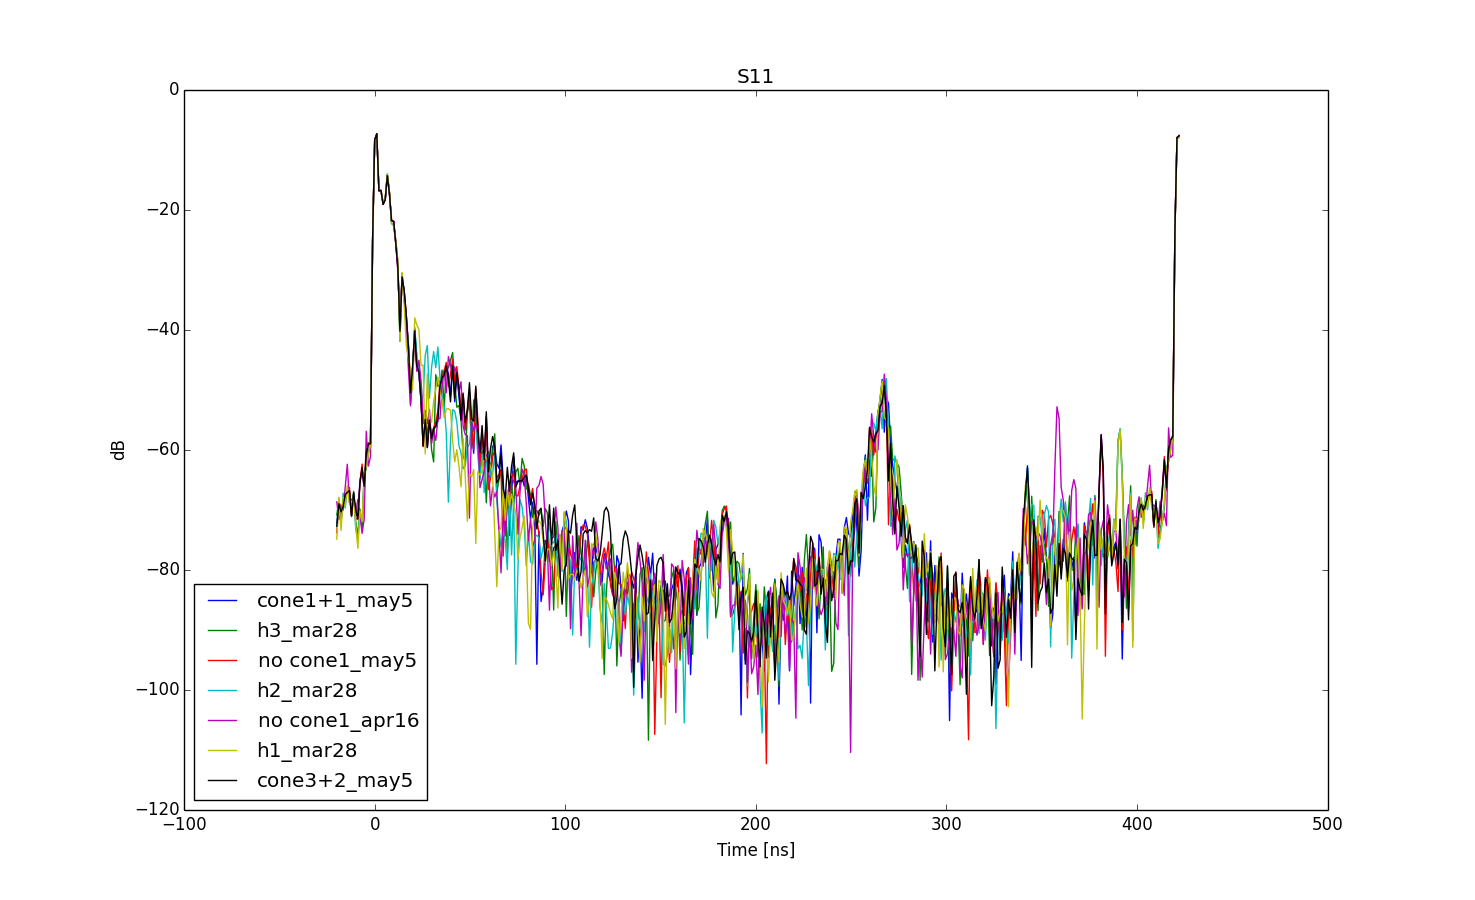
\includegraphics[width =\textwidth]{reflectometry_plots/configcompare}
	\caption{Shows mar28 height tests, apr16, may5 cone test
\label{Fig:} }
	\end{center}
\end{figure}
\begin{figure}[H]
	\begin{center}
	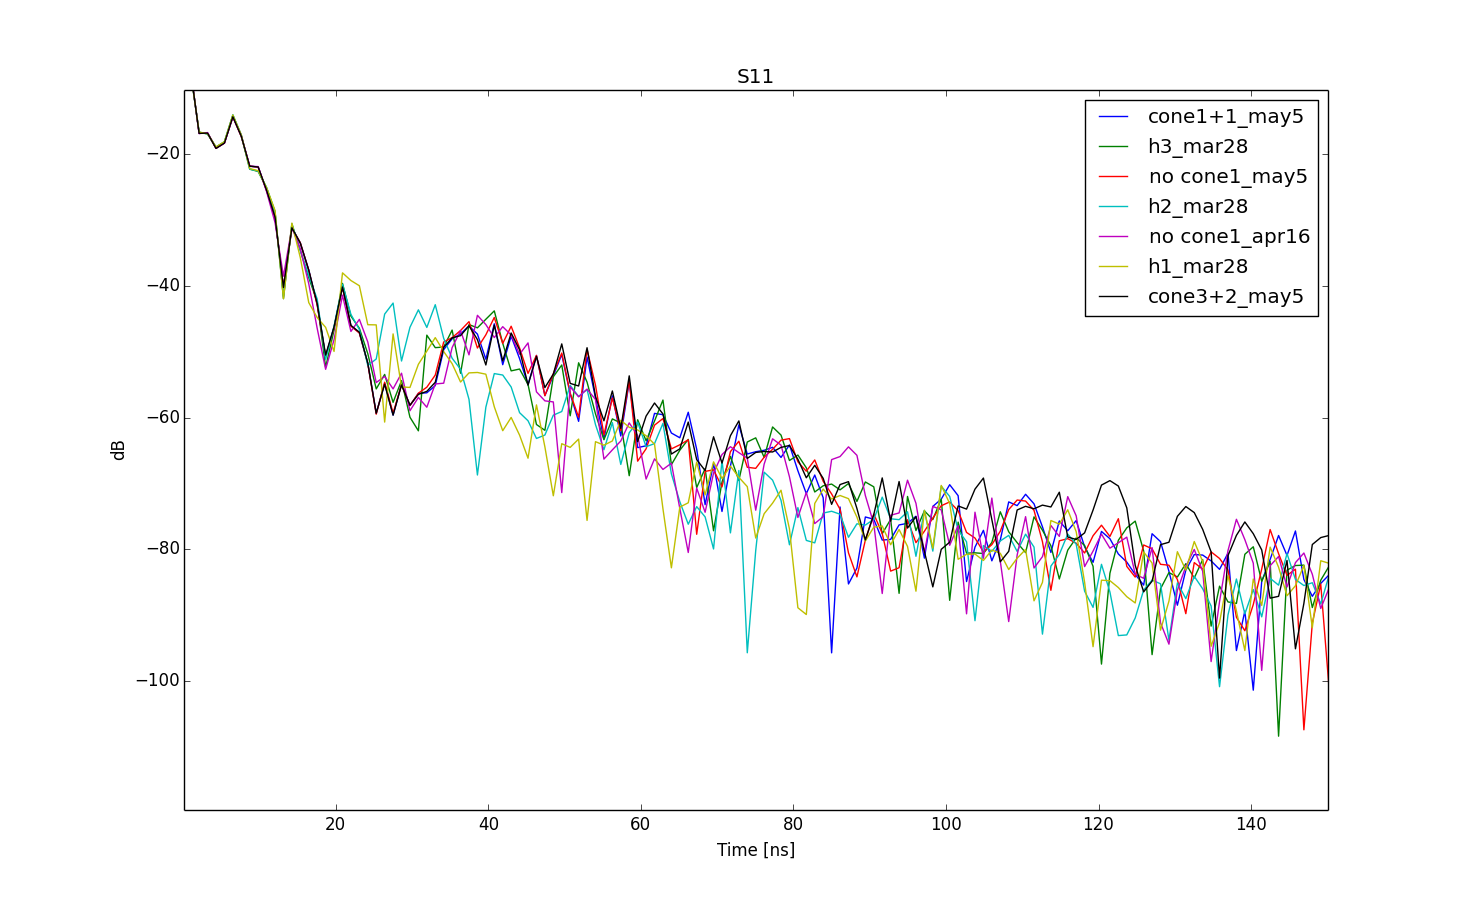
\includegraphics[width =\textwidth]{reflectometry_plots/configcompare10-150ns}
	\caption{Shows mar28 height tests, apr16, may5 cone test zoomed on 10-150ns, can see height test changed the delay
\label{Fig:} }
	\end{center}
\end{figure}

\begin{figure}[H]
	\begin{center}
	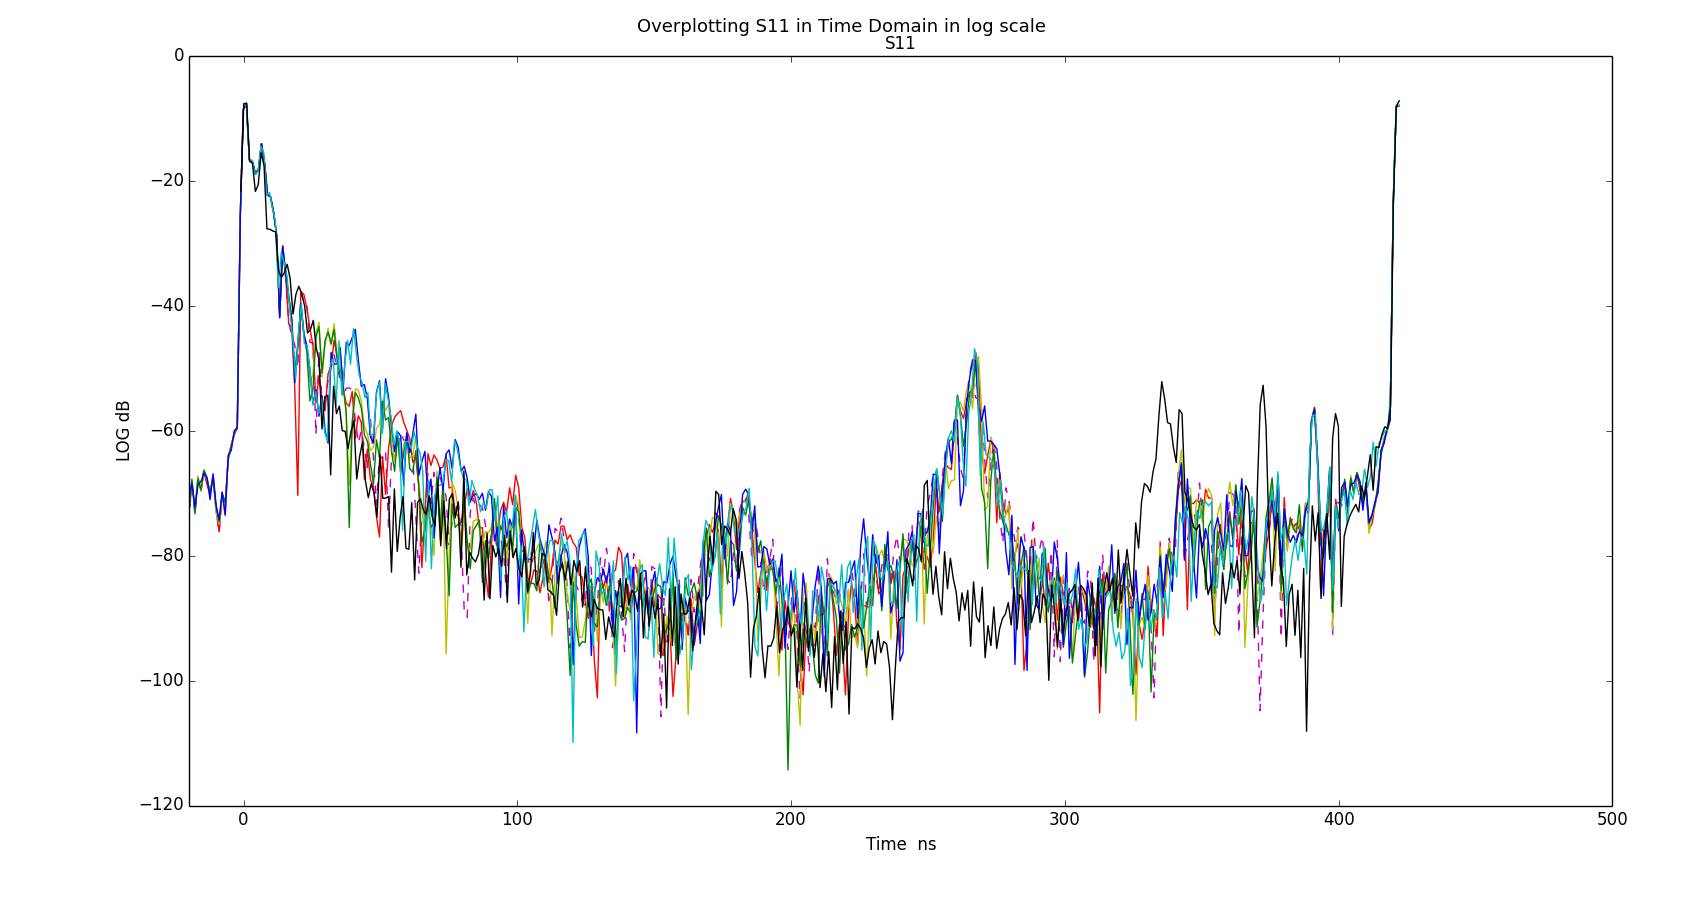
\includegraphics[width =\textwidth]{reflectometry_plots/Mar28/s11all-mar28mix17set1}
	\caption{Shows mar28 height tests, apr16, may5 cone test and test not on dish, shows bump is reflection due to surroundings.
\label{Fig:} }
	\end{center}
\end{figure}

May 5th stuff
@ height 14' 6"
mountain bumps ~ 60' - 80'

Dish without cone, with screen
set1- set2: measurements without cone, 2 metal sheets covering the entrace to the dish, covering panel A, B
set5- set6: measurements with cone, 2 metal sheets covering the entrance to the dish, covering panel A, B

\begin{figure}[H]
	\begin{center}
	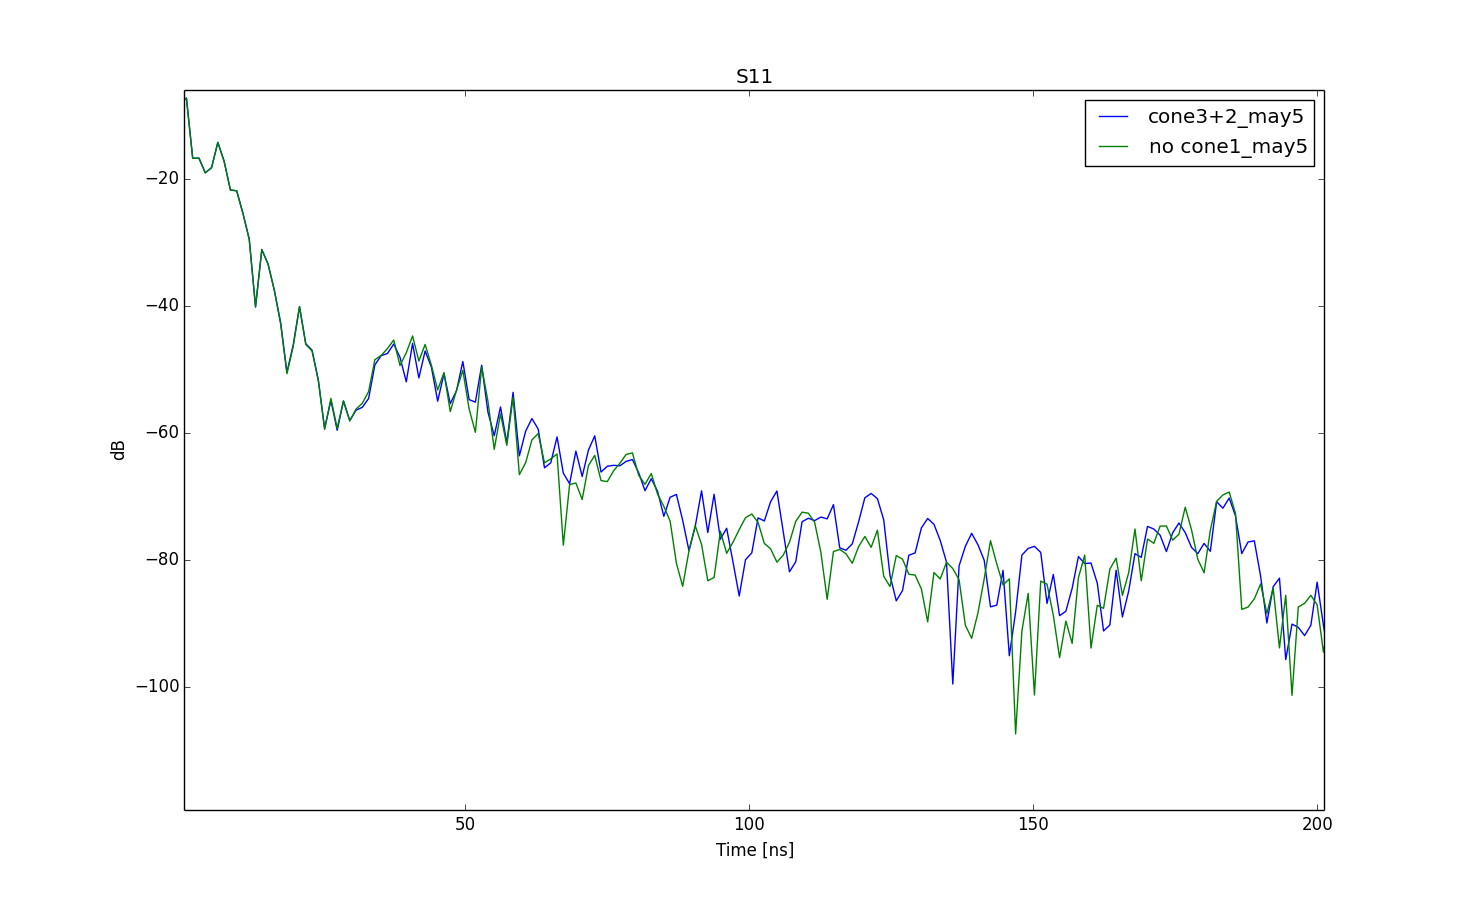
\includegraphics[width =\textwidth]{reflectometry/May5/set1vsset3zoom}
	\caption{CONFIG 1
\label{Fig:} }
	\end{center}
\end{figure}
=====

April 16
@ 14'3" 
no_cone1 = containing data taken without cone with 1 metal sheet
@14'6"
set3- set4: measuremnets with cone, 1 metal sheet covering the entrance to the dish, covering panel A
\begin{figure}[H]
	\begin{center}
	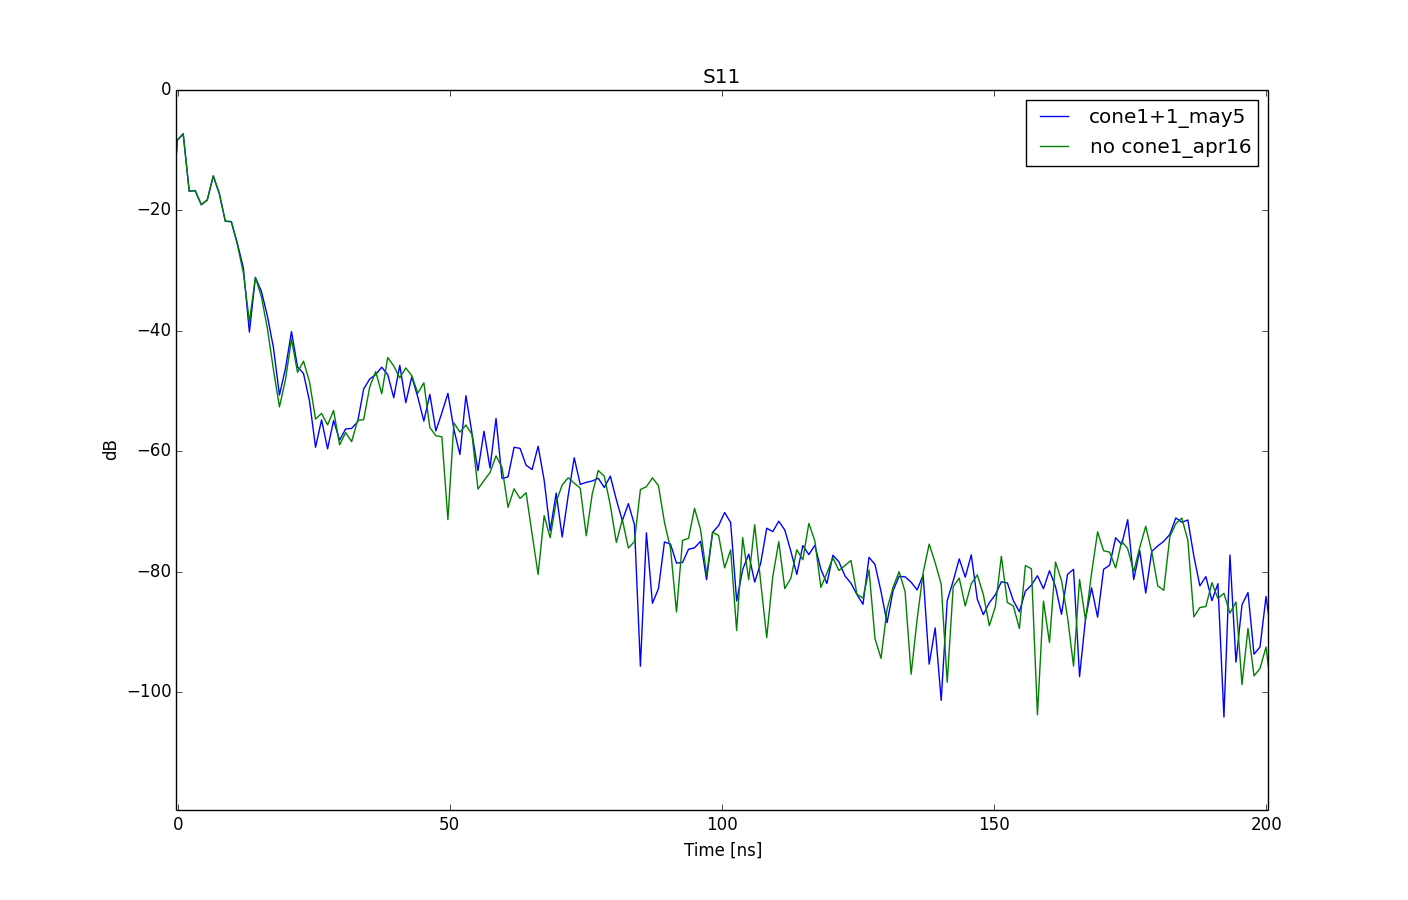
\includegraphics[width =\textwidth]{reflectometry/May5/nocone_vs_set3zoom}
	\caption{CONFIG 2
\label{Fig:} }
	\end{center}
\end{figure}

\begin{figure}[H]
	\begin{center}
	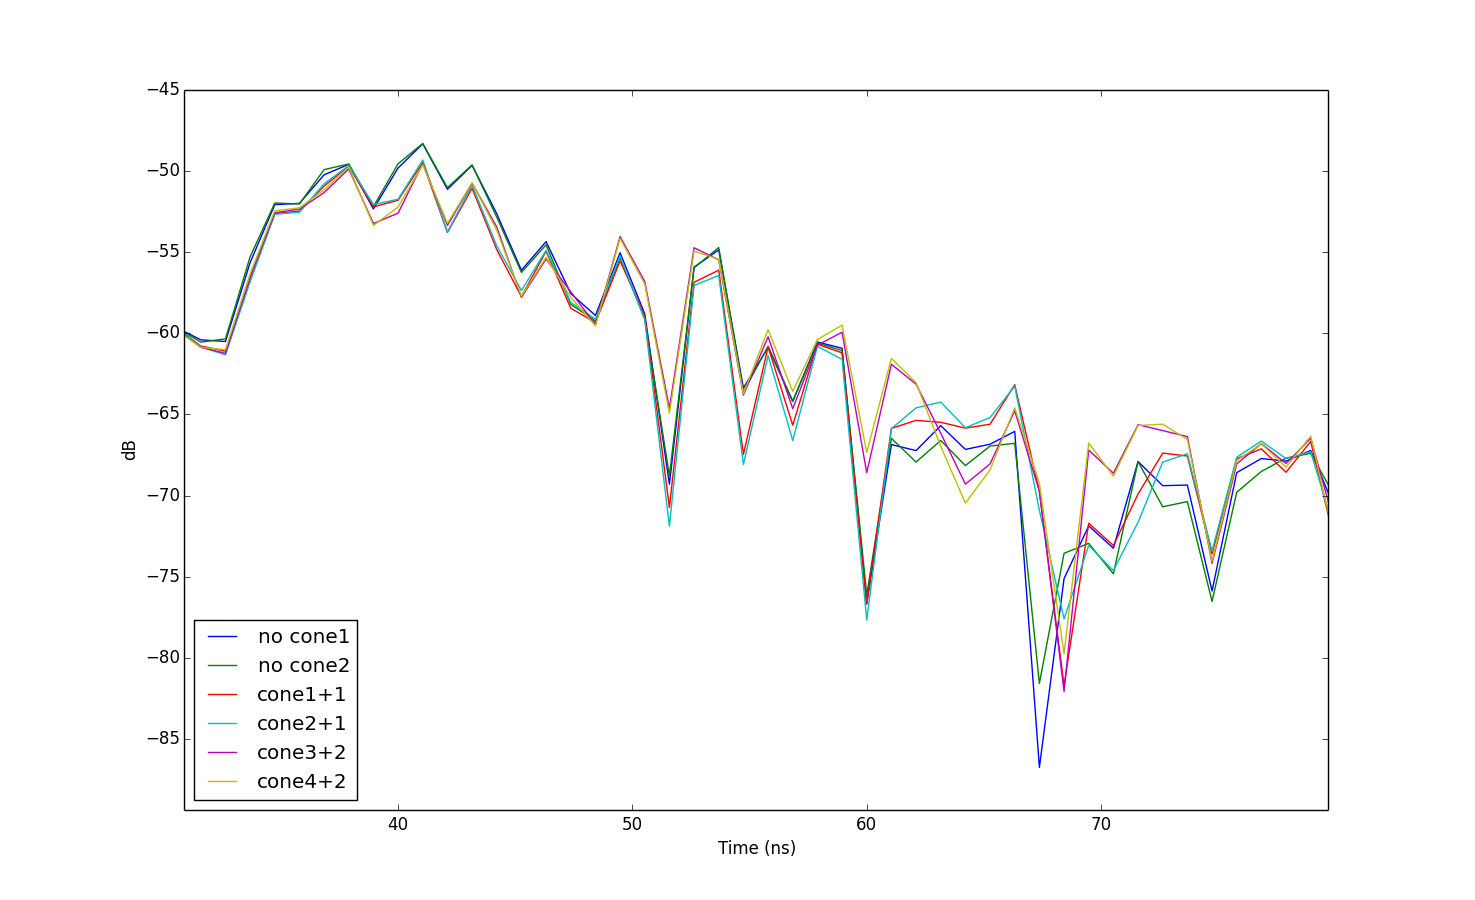
\includegraphics[width =\textwidth]{reflectometry/May5/S11_1st2nd_refl}
	\caption{Shows cone VS no cone, combine 2 plots above, apparent difference cone make, but needs redesign for better backlobe minimization as seen from ~48ns.
\label{Fig:} }
	\end{center}
\end{figure}

========
dish different heights
Mar 28
h1 = 67"
h2 = 10'3.5"
h3 = 14'0.5"

\begin{figure}[H]
	\begin{center}
	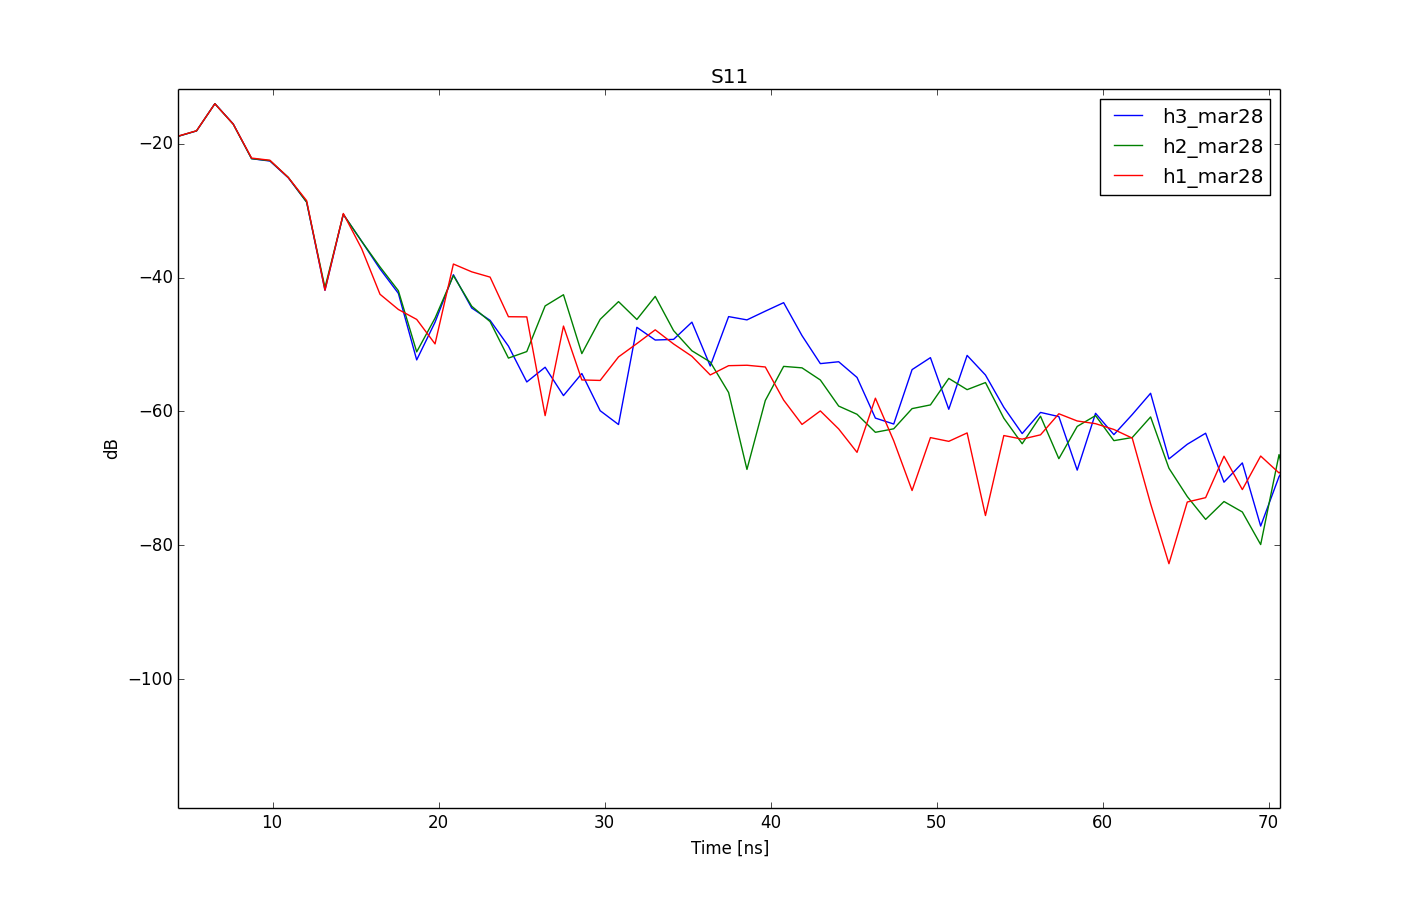
\includegraphics[width =\textwidth]{reflectometry_plots/Mar28/height_test_zoom}
	\caption{height test zoomed
\label{Fig:} }
	\end{center}
\end{figure}


\subsection{Cone test}
> show May 5th cone helped on reduce backlobe, see section \ref{label:reflect}

\subsection{How well did we place everything}
>See contruction_journal

\begin{itemize}
\item delay spectrum for configurations
\item cost
\item photos of constructed element
\item XXX hook up receiver and to a sky test?
\item measured parabolicity
\item why were we right in the antenuation per reflection?
\item does the cone help?
\item how well did we place everything?
\item ways to ensure spec in field
\item mention extender as unnecessary in flat deployments
\end{itemize}

\section{Conclusion}
\label{sec:conclusion}

\begin{itemize}
\item relevance to HERA, project cost
\item link Pober et al. (2014) sensitivity/science
\item polarization matching
\item frequency coverage, need for a feed re-design.
\end{itemize}

\section{Acknowledgment}

We would like to thank SKA-SA for the site infrastructure, maintenance, and observing support
that has made this work possible, as well as the significant efforts of the staff at
NRAO's Green Bank and Charlottesville sites.  AP would like to thank M. McQuinn and A. Lidz
for helpful discussions and ionization models.
The PAPER project is supported
by the National Science Foundation (awards 0804508,
1129258, and 1125558), and a generous grant
from the Mt. Cuba Astronomical Association.

% ---------------------------------------------------------------------
% ---------------------------------------------------------------------
% ---------------------------------------------------------------------

\bibliographystyle{apj}
\bibliography{biblio}

\end{document}

\begin{figure}[H]
	\begin{center}
	\includegraphics[width =\textwidth]{}
	\caption{
\label{Fig:} }
	\end{center}
\end{figure}
